\documentclass{scrreprt}

\usepackage{aligned-overset}
\usepackage{amsmath}
\usepackage{amsthm}
\usepackage{amssymb}
\usepackage{bm}
\usepackage[shortlabels]{enumitem}
\usepackage{hyperref}
\usepackage[utf8]{inputenc}
\usepackage{multicol}
\usepackage{mathtools}
\usepackage{pdflscape}
\usepackage{physics}
\usepackage{polynom}
\usepackage{tabularx}
\usepackage[table]{xcolor}
\usepackage{titling}
\usepackage{fancyhdr}
\usepackage{xfrac}
\usepackage{pgfplots}

\pgfplotsset{compat = newest}
\usetikzlibrary{arrows, arrows.meta}
\usetikzlibrary{calc}

\author{Karsten Lehmann \\ 4935758}
\date{WiSe 2024/25}
\title{Nachbereitungsaufgaben 9\\INF-B-110, Diskrete Strukturen}

\setlength{\headheight}{26pt}
\pagestyle{fancy}
\fancyhf{}
\lhead{\thetitle}
\rhead{\theauthor}
\lfoot{\thedate}
\rfoot{Seite \thepage}

\newcommand{\ggT}[0]{\text{ggT}}
\DeclarePairedDelimiter{\floor}{\lfloor}{\rfloor}

\begin{document}
\paragraph{N9}
\begin{enumerate}[(a)]
\item Von einem Graphen $G = \qty\big(V, E)$ ist bekannt, dass er genau 61 Knoten
  besitzt und sein Komplement $\overline{G}$ ein Baum ist.
  Berechnen Sie die Anzahl an Kanten von $G$.

  \subparagraph{Lsg.} Da $\overline{G}$ ein Baum ist, folgt
  \[
    \abs{E\qty\big(\overline{G})}
    = \abs{V\qty\big(\overline{G})} - 1 = 61 - 1 = 60
  \]
  Nun sind die Möglichen Kanten von G $\binom{V}{2}$ mit
  $\abs{\binom{V}{2}} = \binom{61}{2} = 1830$.
  Nun ist $E\qty\big(G) = \binom{V}{2} \setminus E\qty\big(\overline{G})$ mit
  $\abs{E\qty\big(G)} = \abs{\binom{V}{2}} - \abs{E\qty\big(\overline{G})}
  = 1830 - 60 = 1770$.

\item Bei einem lokalen Schachturnier treten 4 Personen mit Namen A, B, C, und D
  gegeneinander an.
  Jede Person spielt einmal gegen jede der anderen Personen.
  Es darf jedoch niemand mehr als an Spiel an einem Tag spielen.
  \begin{enumerate}[(1)]
  \item Stellen Sie die Situation durch einen Graphen dar.
    Dabei sollen die Knoten die Spiele bezeichnen und zwischen zwei Knoten ist
    genau dann eine Kante, wenn es eine Person gibt, die bei beiden Spielen
    mitspielt.
    Geben Sie ein Diagramm dieses Graphen an.

    \subparagraph{Lsg.} Die Knoten sind mit der zwei-Elementigen Menge der
    Teilnehmer eines Spiels bezeichnet:

    \begin{tikzpicture}
      \node[circle, draw, inner sep=0pt, minimum size=1mm,label=below:{$\qty\big{A, B}$}] (ab) at (0,0) {};
      \node[circle, draw, inner sep=0pt, minimum size=1mm,label=below:{$\qty\big{A, C}$}] (ac) at (2,0) {};
      \node[circle, draw, inner sep=0pt, minimum size=1mm,label=right:{$\qty\big{A, D}$}] (ad) at ($(3, {sqrt(3)})$) {};
      \node[circle, draw, inner sep=0pt, minimum size=1mm,label=above:{$\qty\big{B, C}$}] (bc) at ($(2, {2*sqrt(3)})$) {};
      \node[circle, draw, inner sep=0pt, minimum size=1mm,label=above:{$\qty\big{B, D}$}] (bd) at ($(0, {2*sqrt(3)})$) {};
      \node[circle, draw, inner sep=0pt, minimum size=1mm,label=left:{$\qty\big{C, D}$}] (cd) at ($(-1, {sqrt(3)})$) {};

      \draw (ac) -- (bc) -- (ab) -- (ac) -- (ad) -- (cd) -- (bc);
      \draw (ac) -- (cd) -- (bd) -- (ab) -- (ad) -- (bd) -- (bc);
    \end{tikzpicture}

  \newpage
  \item Untersuchen Sie, wie viele Farben nötig sind, um die Knoten des Graphen
    so zu färben, dass keine zwei benachbarten Knoten dieselbe Farbe haben.

    \subparagraph{Lsg.} Der Graph hat leicht zu erkennen einen ungeraden Kreis
    $\qty\big{A, B} \leftrightarrow \qty\big{A, D} \leftrightarrow \qty\big{B, D}$.
    Somit ist er schon mal nicht zweifärbbar.
    Allerdings findet schnell ein Lösung mit drei Farben:

    \begin{tikzpicture}
      \node[circle, draw, fill, red, inner sep=0pt, minimum size=2mm,label=below:{$\qty\big{A, B}$}] (ab) at (0,0) {};
      \node[circle, draw, fill, blue, inner sep=0pt, minimum size=2mm,label=below:{$\qty\big{A, C}$}] (ac) at (2,0) {};
      \node[circle, draw, fill, green, inner sep=0pt, minimum size=2mm,label=right:{$\qty\big{A, D}$}] (ad) at ($(3, {sqrt(3)})$) {};
      \node[circle, draw, fill, green, inner sep=0pt, minimum size=2mm,label=above:{$\qty\big{B, C}$}] (bc) at ($(2, {2*sqrt(3)})$) {};
      \node[circle, draw, fill, blue, inner sep=0pt, minimum size=2mm,label=above:{$\qty\big{B, D}$}] (bd) at ($(0, {2*sqrt(3)})$) {};
      \node[circle, draw, fill, red, inner sep=0pt, minimum size=2mm,label=left:{$\qty\big{C, D}$}] (cd) at ($(-1, {sqrt(3)})$) {};

      \draw (ac) -- (bc) -- (ab) -- (ac) -- (ad) -- (cd) -- (bc);
      \draw (ac) -- (cd) -- (bd) -- (ab) -- (ad) -- (bd) -- (bc);
    \end{tikzpicture}

  \item Wie viele Spieltage sind mindestens nötig?
    Begründen Sie Ihre Antwort!

    \subparagraph{Lsg.}  Wenn zwei Knoten verbunden sind, dann können sie in
    der vorherigen Teilaufgabe nicht die selbe Farbe haben.
    Und zwei Knoten (Spiele) sind genau dann verbunden, wenn ein Spieler an
    beiden beteiligt ist.
    Somit können an jedem Spieltag nur Spiele mit der selben Farbe - also
    unterschiedlichen Spielern - stattfinden.
    Da in der vorherigen Teilaufgabe bereits gezeigt wurde, dass mindestens 3
    Farben benötigt werden, müssen somit auch mindestens 3 Spieltage eingeplant
    werden.
  \end{enumerate}
\end{enumerate}
\end{document}
